\section{Tests}
\subsection{Klebeversuch}
\begin{tabular}{p{3.6cm}p{\textwidth-3.6cm-0.7cm}}
    \rule{0pt}{11pt}\textit{Typ}              & Klebeversuch \\ 
    \rule{0pt}{11pt}\textit{Datum}:           & 06.03.2015   \\
    \rule{0pt}{11pt}\textit{Ort}:             & Teaminsel \\
    \rule{0pt}{11pt}\textit{Tester}:          & Matteo Trachsel \\
    \rule{0pt}{11pt}\textit{Ziel des Testes}: & Das Ziel dieses Testes bestand darin, den 
    gekauften Kleber UHU Hart auf seine Klebekraft und auf sein Erscheinungsbild zu testen. \\
    \rule{0pt}{11pt}\textit{Aufbau / Ablauf}: & 
    Für den Test werden verschiedene Acrylglas-Stücke zusammengeklebt.
    Hierfür wird der Kleber wie auf der Gebrauchsanweisung auf zwei Verfahren getestet. 
    Im ersten Versuch wird der UHU Kleber aufgetragen und die zwei Platten zusammengeklebt. 
    Im zweiten Versuch wird der Kleber zuerst auf die Acrylglasstücke aufgetragen und 
    gewartet bis er angetrocknet ist, danach noch einmal eine Schicht vom Kleber aufgetragen 
    und zusammengefügt.\\
    \rule{0pt}{11pt}\textit{Fazit / Verbesserungs-\newline vorschlag}: & 
    Mit dem Versuch konnte gezeigt werden, dass der Kleber sicher glasklar bleibt. Weiter 
    ist die erwünschte Klebekraft bestätigt worden. Beim zweiten Versuch, wo zuerst der 
    Kleber etwas angetrocknet wurde, ist eine deutlich schlechtere Klebekraft festgestellt 
    worden. Dadurch wird der Kleber immer sofort aufgeklebt.\\
\end{tabular}

\begin{figure}[h!]
	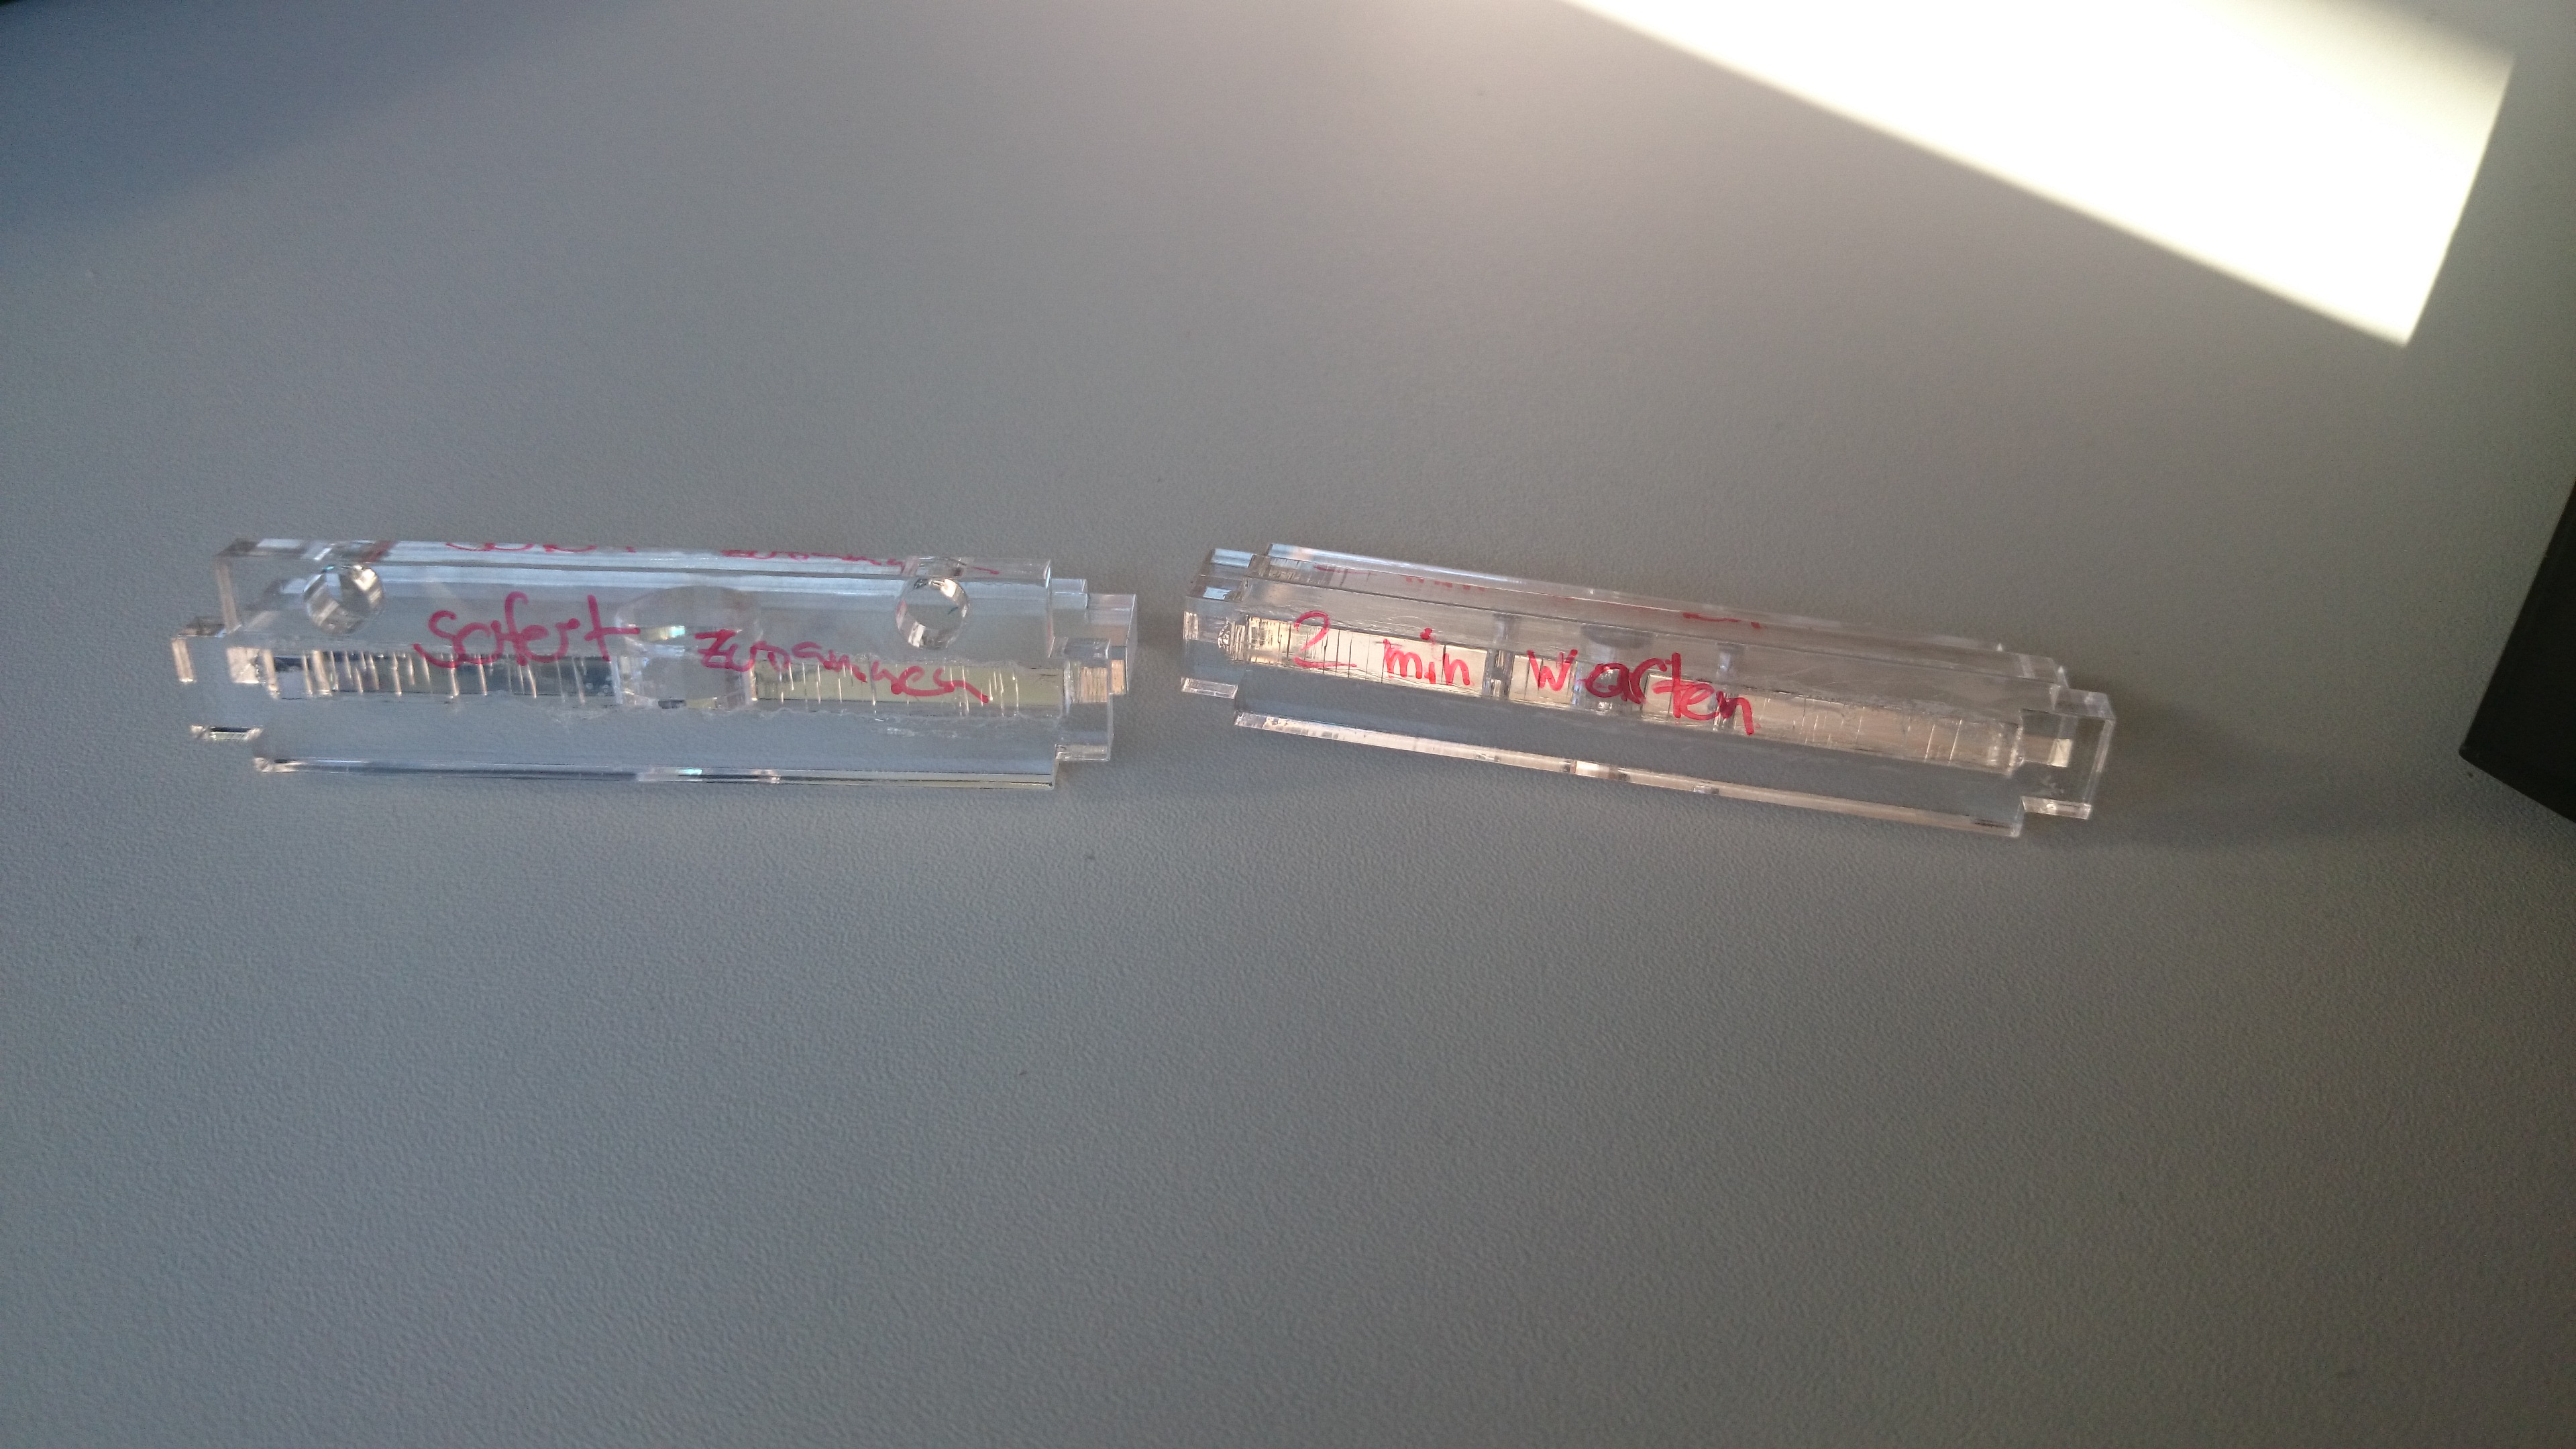
\includegraphics[width=0.7\textwidth,clip,trim=0cm 0cm 0cm 0cm]
	{Testberichte/Klebeversuch.jpg}
	\centering
	\caption{Klebeversuch mit UHU Kleber} 
	\label{abb:Klebeversuch}
\end{figure}